%texexptitled======================================================================
% lab1-gcd
%-----------------------------------------------------------------------
%

\documentclass[11pt]{article}

% Package includes

\usepackage{graphicx}
\usepackage{color}
\usepackage{comment}
\usepackage{multirow}
\usepackage{askmaps}
\usepackage{amssymb}
\usepackage{amsmath}
\usepackage{tikz}
\usepackage{circuitikzgit}
\usetikzlibrary{arrows, positioning, shapes.geometric, circuits.logic.US}
\tikzstyle{line}=[draw]
\tikzstyle{arrow}=[draw, -latex]

% Wrap long URLs with hyphens
\PassOptionsToPackage{hyphens}{url}\usepackage{hyperref}
\usepackage{pdftexcmds}
\usepackage{upquote}
\usepackage{textcomp}
\usepackage{minted}
\usepackage[listings]{tcolorbox}
\usepackage{enumerate}
\usepackage{enumitem}
\usepackage{mathtools}
\DeclarePairedDelimiter{\ceil}{\Big\lceil}{\Big\rceil}

\tcbset{
texexp/.style={colframe=black, colback=lightgray!15,
         coltitle=white,
         fonttitle=\small\sffamily\bfseries, fontupper=\small, fontlower=\small},
     example/.style 2 args={texexp,
title={Question \thetcbcounter: #1},label={#2}},
}

\newtcolorbox{texexp}[1]{texexp}
\newtcolorbox[auto counter]{texexptitled}[3][]{%
example={#2}{#3},#1}

\setlength{\topmargin}{-0.5in}
\setlength{\textheight}{9in}
\setlength{\oddsidemargin}{0in}
\setlength{\evensidemargin}{0in}
\setlength{\textwidth}{6.5in}

% Useful macros

\newcommand{\note}[1]{{\bf [ NOTE: #1 ]}}
\newcommand{\fixme}[1]{{\bf [ FIXME: #1 ]}}
\newcommand{\wunits}[2]{\mbox{#1\,#2}}
\newcommand{\um}{\mbox{$\mu$m}}
\newcommand{\xum}[1]{\wunits{#1}{\um}}
\newcommand{\by}[2]{\mbox{#1$\times$#2}}
\newcommand{\byby}[3]{\mbox{#1$\times$#2$\times$#3}}


\newenvironment{tightlist}
{\begin{itemize}
 \setlength{\parsep}{0pt}
 \setlength{\itemsep}{-2pt}}
{\end{itemize}}

\newenvironment{titledtightlist}[1]
{\noindent
 ~~\textbf{#1}
 \begin{itemize}
 \setlength{\parsep}{0pt}
 \setlength{\itemsep}{-2pt}}
{\end{itemize}}

% Change spacing before and after section headers

\makeatletter
\renewcommand{\section}
{\@startsection {section}{1}{0pt}
 {-2ex}
 {1ex}
 {\bfseries\Large}}
\makeatother

\makeatletter
\renewcommand{\subsection}
{\@startsection {subsection}{1}{0pt}
 {-1ex}
 {0.5ex}
 {\bfseries\normalsize}}
\makeatother

% Reduce likelihood of a single line at the top/bottom of page

\clubpenalty=2000
\widowpenalty=2000

% Other commands and parameters

\pagestyle{myheadings}
\setlength{\parindent}{0in}
\setlength{\parskip}{10pt}

% Commands for register format figures.

\newcommand{\instbit}[1]{\mbox{\scriptsize #1}}
\newcommand{\instbitrange}[2]{\instbit{#1} \hfill \instbit{#2}}

\newif\ifsolution

\if\issolution1
\newenvironment{solution}
    {\color{red}}
    {\color{black}}
\solutiontrue
\else
\excludecomment{solution}
\solutionfalse
\fi


\graphicspath{{./figs/}}


%-----------------------------------------------------------------------
% Document
%-----------------------------------------------------------------------

\begin{document}
\def\PYZsq{\textquotesingle}


\newcommand{\headertext}{EE142 Problem Set 7}
\renewcommand{\thesubsection}{\thesection.\alph{subsection}}

\title{\vspace{-0.4in}\Large \bf \headertext \vspace{-0.1in}}
\author{Vighnesh Iyer}

\date{\today}
\maketitle

\markboth{\headertext}{\headertext}
\thispagestyle{empty}

\section{Noise Figure of Cascade Blocks and Lossy Transmission Line}
\begin{enumerate}[label=(\alph*)]
    \begin{figure}[H]
        \centering 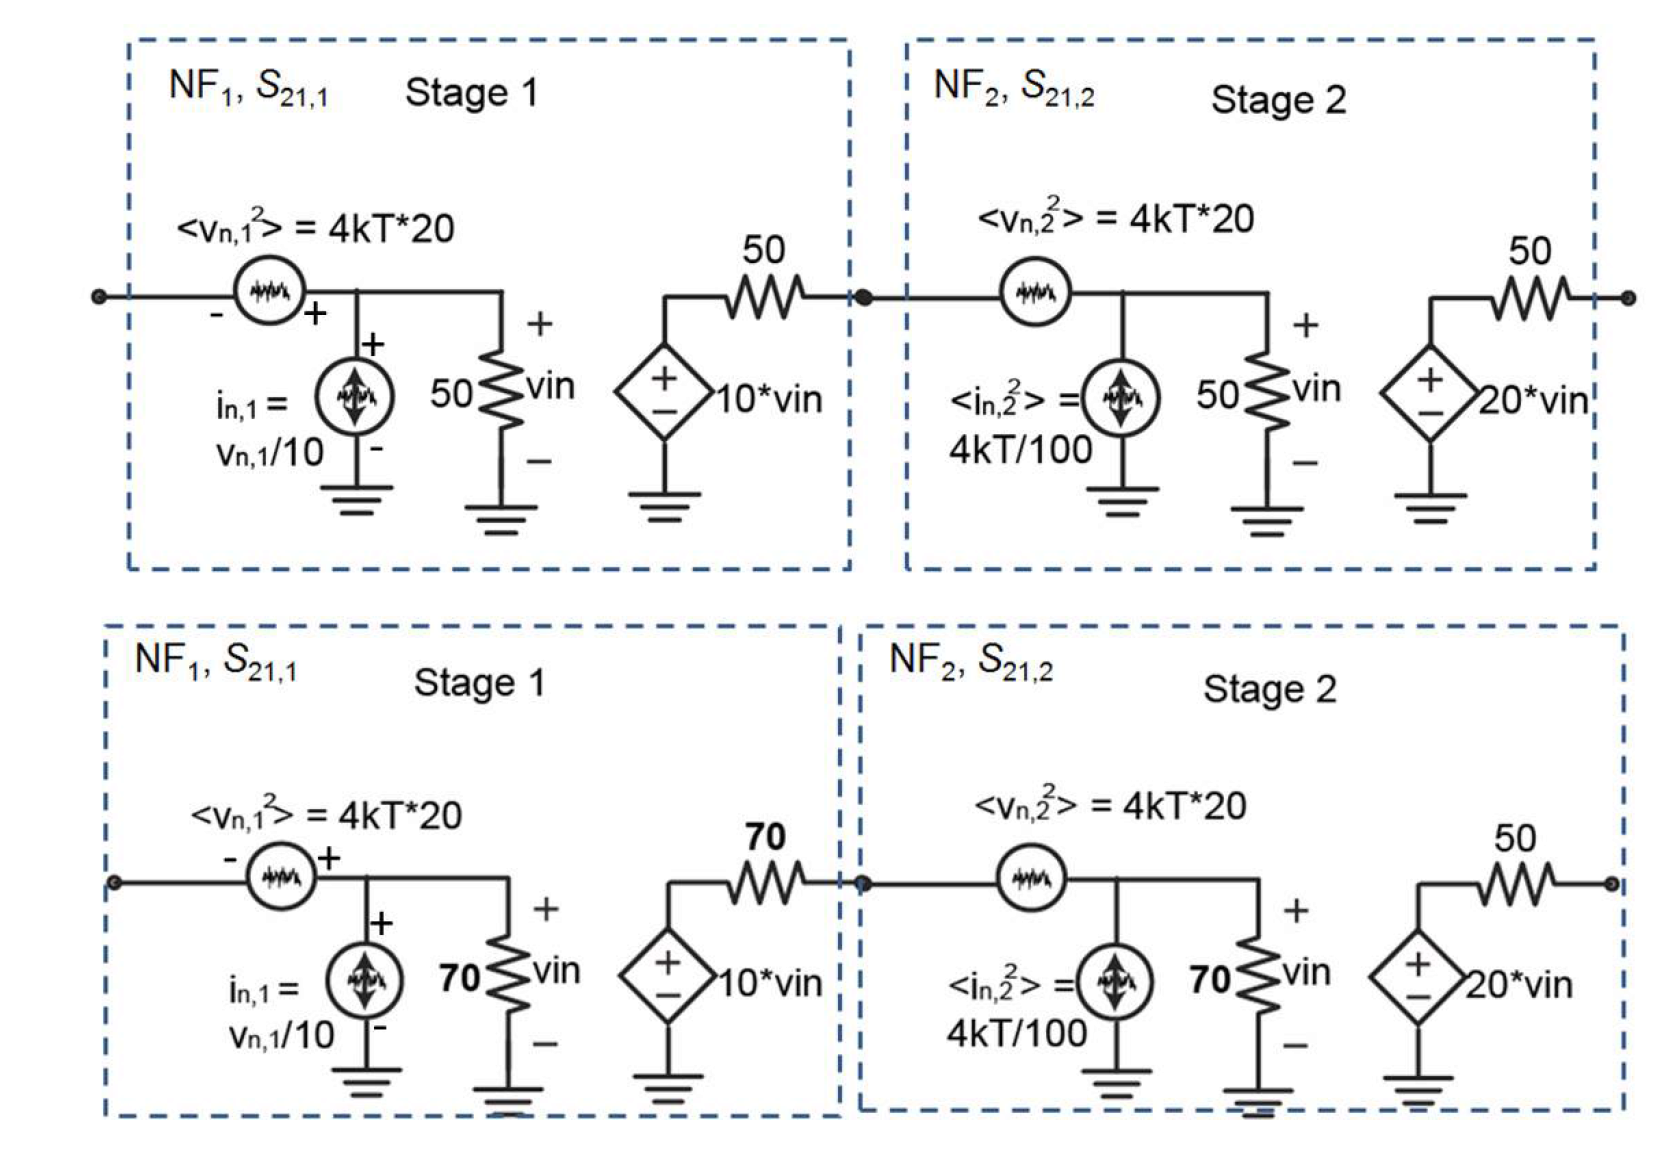
\includegraphics[width=\textwidth-2cm]{problem1a_schematic.png}
    \end{figure}

    \item {\color{blue}For the above two cascade circuits, calculate the power gains and noise figures for each stage (i.e. $S_{21,1}$, $S_{21,2}$, $NF_1$, $NF_2$) and the two stage circuits ($S_{21,total}$, $NF_{total}$).
    The resistors are assumed to be noiseless.}

    \subsection{Cascade 1 - S}
    \begin{align*}
        S_{21,1} &= 5 \\
        S_{21,2} &= 10 \\
        S_{21,total} &= 50
    \end{align*}

    We assumed $Z_0$ is $50 \Omega$. We drive the input with a 50 $\Omega$ AC source and terminate the output with a $50 \Omega$ load.
    These values represent voltage and power gain due to equal input/output impedances.

    \subsection{Cascade 1 - Noise}

    For the first cascase's stage 1, we begin by input referring the noise sources and collapsing the voltage and current noise into $\overline{v_{eq}^2}$.
    From lecture:

    \begin{align*}
        \overline{v_{eq}^2} &= \overline{v_n^2} + \overline{i_n^2} R_s^2 \text{ for uncorrelated noise} \\
        \overline{v_{eq}^2} &= \overline{v_n^2} |1 + Y_c Z_s|^2 + |Z_s|^2 \overline{i_u^2} \text{ for correlated noise} \\
        \text{ where } i_c &= Y_c V_n \text{ and } i_n = i_c + i_u \\
        \text{ then } F &= 1 + \frac{N_{amp,i}}{N_s} = 1 + \frac{\overline{v_{eq}^2}}{\overline{v_s^2}}
    \end{align*}

    Assume we are calculating noise figure in a $50 \Omega$ environment, $R_s = 50 \Omega$ and $\overline{v_s^2} = 4 kT R_s$.
    We assume that all noise sources represented are defined as \emph{spot noise}.
    Furthermore, we \emph{don't} assume that $\overline{v_n^2}$ and $\overline{i_n^2}$ are uncorrelated, and include covariance terms when needed.

    \begin{align*}
        F_1 &= 1 + \frac{\overline{v_{eq,1}^2}}{\overline{v_s^2}} = 1 + \frac{4kT\cdot 20 |1 + 0.1 \cdot 50|^2}{4kT \cdot 50} = 15.4 \\
        NF_1 &= 10 \cdot \log(F_1) = 11.88 \text{ dB} \\
        F_2 &= 1 + \frac{\overline{v_{eq,1}^2}}{\overline{v_s^2}} = 1 + \frac{4kT \cdot 20 + 4kT \cdot \frac{1}{100} \cdot 50^2}{4kT \cdot 50} = 1.9 \\
        NF_2 &= 2.79 \text{ dB} \\
        F_{tot} &= F_1 + \frac{F_2 - 1}{G_1} = 15.4 + \frac{1.9-1}{5^2} = 15.436 \\
        NF_{tot} &= 11.885 \text{ dB}
    \end{align*}

    where we recognize that all current noise is correlated to the voltage noise. Furthermore, we can use Friis' cascade noise formula due to internally matched impedances.

    \subsection{Cascase 2 -S}
    \begin{align*}
        S_{21,1} &= \frac{V_s \frac{70}{70 + 50} \cdot 10 \cdot \frac{50}{50 + 70}}{V_s \frac{70}{70+50}} = 4.147 \\
        S_{21,2} &= \frac{V_s \frac{70}{70 + 50} \cdot 20 \cdot \frac{1}{2}}{V_s \frac{70}{70+50}} = 10 \\
        S_{21,total} &= \frac{V_s \frac{70}{70+50} \cdot 10 \cdot \frac{1}{2} \cdot 20 \frac{1}{2}}{V_s \frac{70}{70+50}} = 50
    \end{align*}

    \subsection{Cascase 2 - Noise}
    \begin{align*}
        F_1 &= 15.4 \text{ same as cascade 1} \\
        F_2 &= 1.9 \text{ same as cascade 1} \\
        F_{tot} &= 15.436
    \end{align*}

    The noise figure of each stage doesn't change because input referring the noise sources doesn't depend on the stages' terminations. The total noise figure also doesn't change since input referring the noise from the second stage still sees a pure gain by 10.

    \item {\color{blue} Is the formula $NF_{total} = NF_1 + \frac{NF_2-1}{|S_{21,1}^2|}$ applicable?}

    This formula is definetely applicable if each stage is impedance matched internally and to the external source resistance and load impedance used in the measurement; otherwise it doesn't apply generally.

    \item {\color{blue} For a lossy transmission line illustrated below, derive its noise figure.}

    \begin{figure}[H]
        \centering 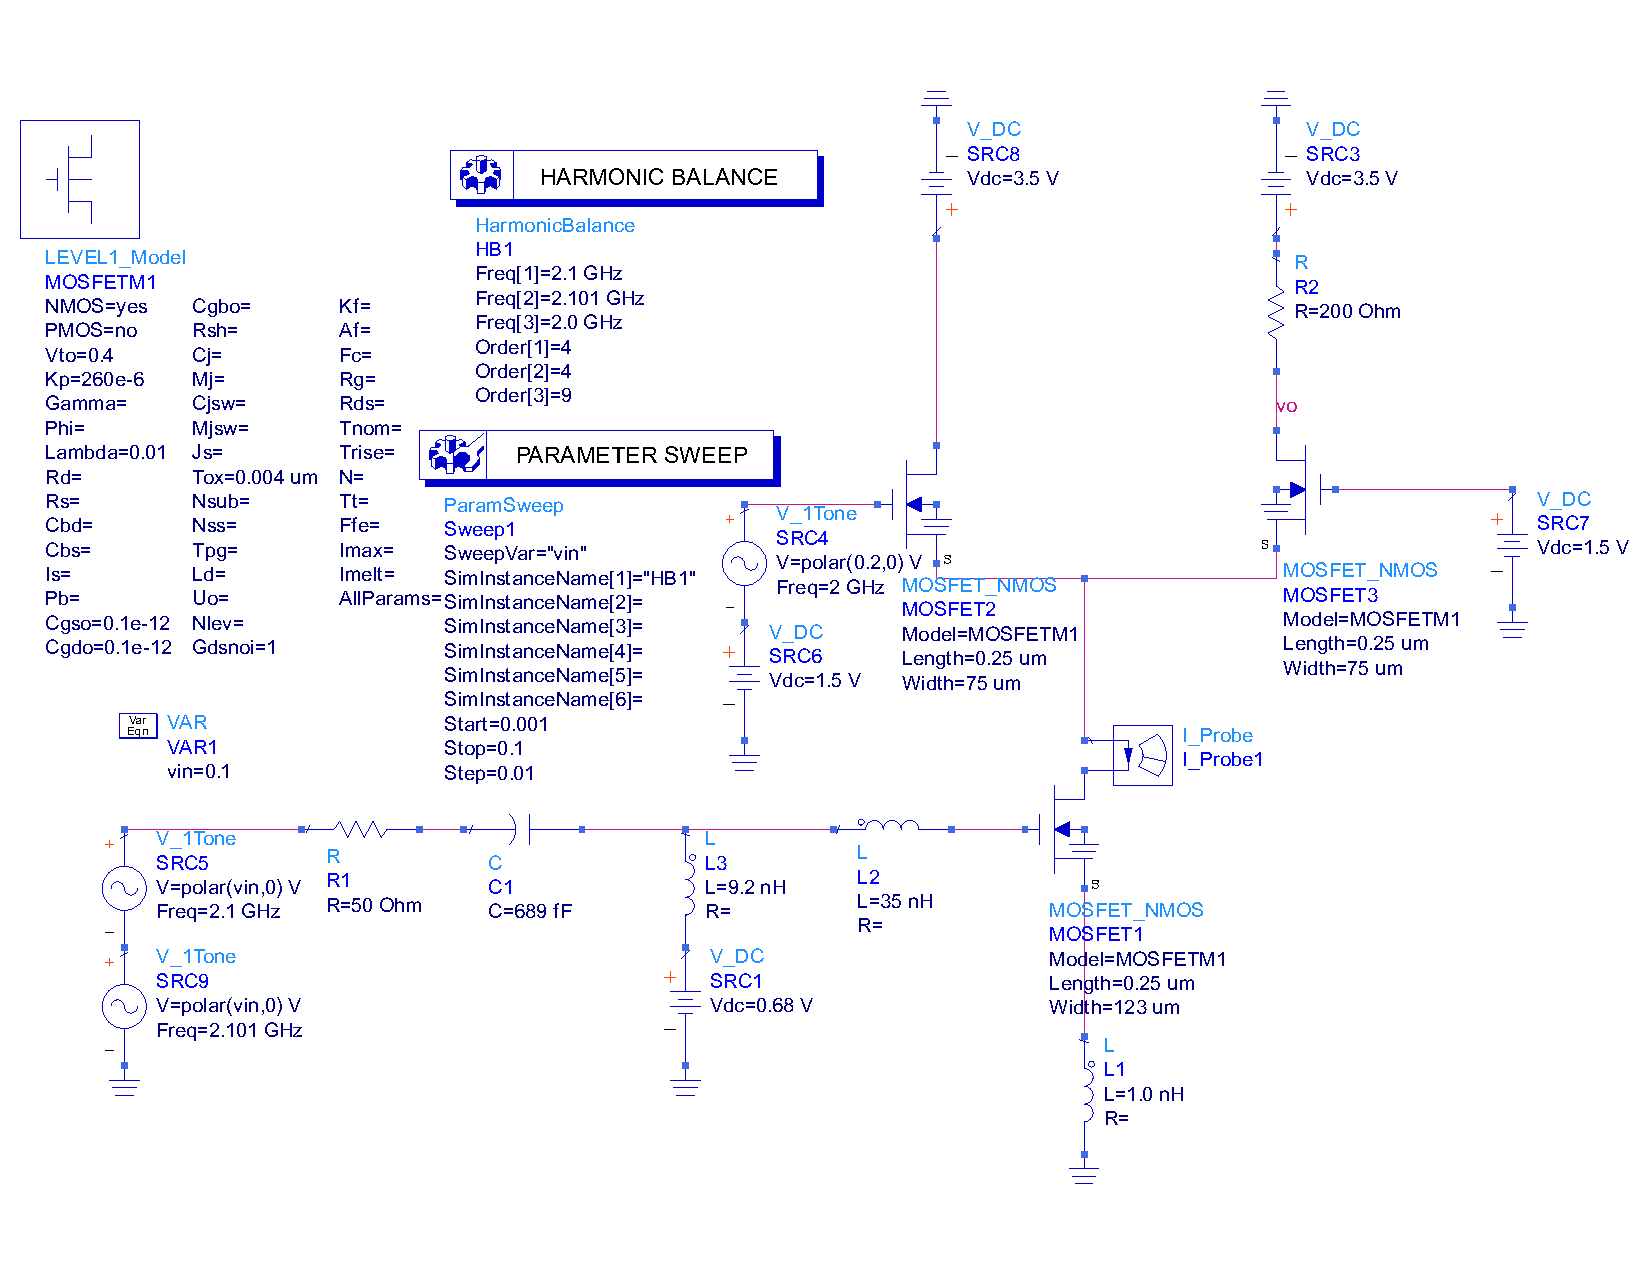
\includegraphics[width=\textwidth-8cm]{problem1c_schematic.png}
    \end{figure}

    Starting with the definition of $F$:

    \begin{align*}
        F &= \frac{SNR_i}{SNR_o} = \frac{P_{sig}/\overline{v_{n,s}^2}}{P_{sig} \cdot \text{ loss} / \overline{v_{n,s}^2} \cdot \text{ loss}^2} \\
        F &= \frac{1}{\text{loss}}
    \end{align*}

    where 'loss' represents the power loss of the transmission line in steady state from input to output. This is simple to compute, assuming that the line is driven with a source impedance of $Z_0$ with a mean squared noise voltage of $4 kT Z_0$ and terminated with a noiseless load of $Z_0$.

    \begin{align*}
        \text{Power @ Load} &= V_+ e^{-\gamma l} \cdot \frac{1}{Z_0} e^{-\gamma l} V_+ \rvert_{l=0} = \frac{V_+^2}{Z_0} \\
        \text{Power @ Source} &= V_+ e^{-\gamma l} \cdot \frac{1}{Z_0} e^{-\gamma l} V_+ \rvert_{l=-l} = \frac{V_+^2 e^{2 \gamma l}}{Z_0} \\
        \text{Power @ Load / Power @ Source} &= e^{-2 \gamma l} \\
        F &= \frac{1}{e^{-2 \gamma l}} = e^{2 \gamma l}
    \end{align*}

    We know the propagation constant $\gamma = \alpha + j \beta$. Because the velocity of the line is at the speed of light, the imaginary term goes to zero and $\gamma$ is dominated by $\alpha$.

    $$ F = e^{2 \alpha_0 L} $$

    The noise figure seems frequency independent, but any real line has $\beta = \frac{2\pi}{\lambda}$.

    \item {\color{blue} If the tline is used to connect the above two cascade circuits to the $50\Omega$ soucrce (e.g. antenna), what will be the new total noise figures.}

    Both noise figures are the same at:

    \begin{align*}
        F_{tot} = 15.436 + \frac{e^{2 \alpha_0 L} - 1}{|S_{21,tot}|^2}
    \end{align*}

    We can use Friis's cascade formula since the $F_{tot}$ of each cascade is the same and $S_{21,tot}$ are also the same, and furthermore the antenna is matched to the transmission line.
\end{enumerate}

\section{Matching for Low Noise Versus Matching for High Gain}
\emph{In this problem, your answers should be functions of frequency.}

\begin{enumerate}[label=(\alph*)]
    \item {\color{blue} For a simplified common-source model shown below (with noise sources drawn) derive the input referred noise voltage and noise current.}
    \begin{figure}[H]
        \centering 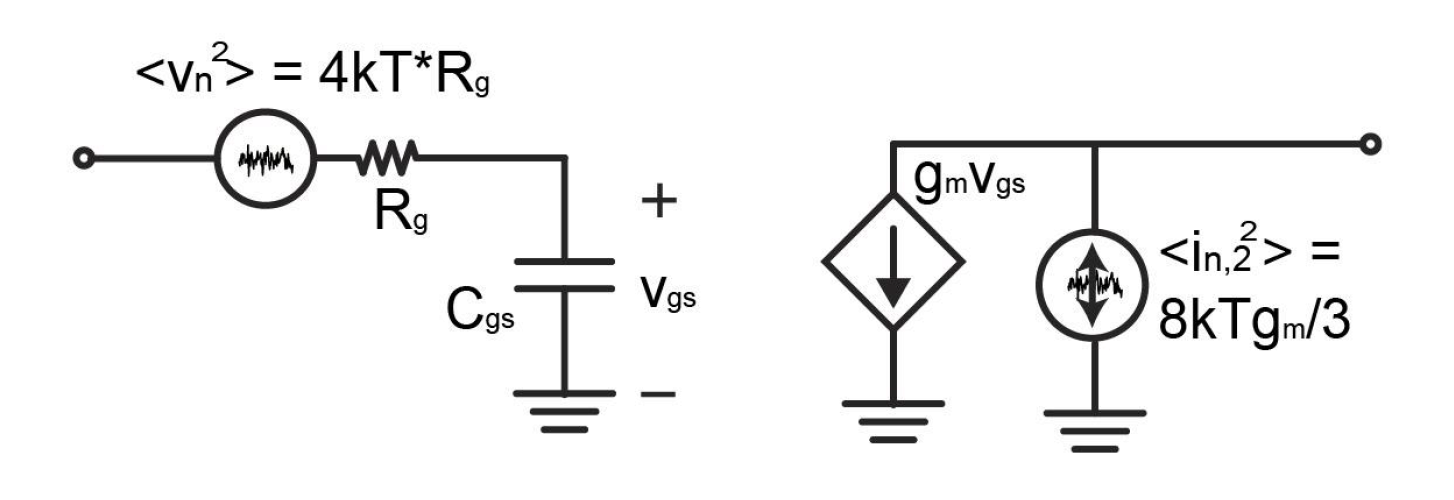
\includegraphics[width=\textwidth-2cm]{problem2a_schematic.png}
    \end{figure}

    Let's first analyze the input RC network to derive the result from lecture. Take the mean squared voltage across the capacitor as $\overline{v_c^2}$.

    \begin{align*}
        \overline{v_c^2} &= \int_{- \infty}^{+ \infty} S(f) |H(f)|^2 df \\
        H(f) &= \frac{1}{1 + RC j \cdot 2 \pi f} \\
        \overline{v_c^2} &= \int^{+\infty}_{-\infty} 2kTR \cdot \frac{1}{(RC 2 \pi f)^2 + 1} df \\
        &= 2kTR \cdot \int^{+\infty}_{-\infty} \frac{1}{(RC 2 \pi f)^2 + 1} df \\
        &= 2kTR \cdot (\frac{\tan^{-1}(RC 2 \pi f)}{RC} \rvert_{- \infty}^{+ \infty}) \\
        &= 2kTR \cdot \frac{1}{2 RC} \\
        &= \frac{kT}{C}
    \end{align*}

    Denote equivalent input current noise as $\overline{i_{n}^2}$ and equivalent input voltage noise as $\overline{v_n^2}$.

    To find equivalent input current noise, first we open the input and measure the output noise.
    \begin{align*}
        \overline{i_{o}^2} &= 8kT g_m / 3
    \end{align*}

    Then remove the noise sources and add a current noise source at the input and again measure the output noise.
    \begin{align*}
        \overline{i_{o}^2} &= \overline{i_n^2} \cdot Z_{gs}^2 \cdot g_m^2
    \end{align*}

    Equating these output noises we find equivalent input current noise:
    \begin{align*}
        \overline{i_n^2} &= \frac{8kT g_m}{3} \cdot \frac{1}{g_m^2 Z_{gs}^2} = \frac{8kT}{3 g_m} \cdot (\omega C_{gs})^2
    \end{align*}

    To find equivalent input voltage noise, first we short the input and measure the output noise.
    \begin{align*}
        \overline{i_{o}^2} &= \frac{kT}{C_{gs}} \cdot g_m^2 + 8kT g_m / 3
    \end{align*}

    The remove the noise sources and add a voltage noise source at the input, measure output noise.
    \begin{align*}
        \overline{i_o^2} &= \overline{v_n^2} \cdot (\frac{Z_{gs}}{Z_{gs} + R_g})^2 \cdot g_m^2
    \end{align*}

    Equating output noises:
    \begin{align*}
        \overline{v_n^2} &= \frac{\frac{kT}{C_{gs}} \cdot g_m^2 + 8kT g_m / 3}{(\frac{Z_{gs}}{Z_{gs} + R_g})^2 \cdot g_m^2} \\
        &= \frac{T k}{3 C_{gs} g_{m}} \left(8 C_{gs} + 3 g_{m}\right) \left(j C_{gs} R_{g} \omega + 1\right)^{2}
    \end{align*}

    Sympy was used to find the equivalent output noise expression (too tedious by hand).

    \item {\color{blue} Following part (a), what is the source impedance that optimizes the noise figure? What is the lowest noise figure?}

    We first decompose $\overline{v_n^2}$ into correlated and uncorrelated parts, and rederive $\overline{v_{eq}^2}$.
    \begin{align*}
        v_n &= v_c + v_u \\
        v_c &= i_n \cdot Z_c \\
        v_{eq} &= i_n \cdot Z_s + i_n \cdot Z_c + V_u = i_n(Z_s + Z_c) + v_u \\
        \overline{v_{eq}^2} &= \overline{i_n^2} |Z_s + Z_c|^2 + \overline{v_u^2}
    \end{align*}

    By expanding $\overline{v_n^2}$ it can be written as:
    \begin{align*}
        \overline{v_n^2} = \overline{i_n^2} \cdot R_{g}^{2} - C_{gs} R_{g}^{2} T \omega^{2} k + \frac{16 i C_{gs} R_{g}}{3 g_{m}} T \omega k + 2 i R_{g} T \omega k + \frac{8 T k}{3 g_{m}} + \frac{T k}{C_{gs}}
    \end{align*}

    We can immediately identify $Z_c = R_g$, and setting $Z_s = R_s$, we can find $\overline{v_{eq}^2}$ symbolically.
    The expression is complicated... not sure if I'm doing something wrong or just not chopping off 'small' terms.

    \begin{align*}
        \overline{v_{eq}^2} = - \frac{8 C_{gs}^{2} T k}{3 g_{m}} \omega^{2} \left(R_{g} + R_{s}\right)^{2} - C_{gs} R_{g}^{2} T \omega^{2} k + \frac{16 i C_{gs} R_{g}}{3 g_{m}} T \omega k + 2 i R_{g} T \omega k + \frac{8 T k}{3 g_{m}} + \frac{T k}{C_{gs}}
    \end{align*}

    Now we can use the standard expression for noise figure:
    \begin{align*}
        F &= 1 + \frac{\overline{v_{eq}^2}}{\overline{v_s^2}} \\
        &= 1 + \frac{1}{4 R_{s} T k} \left(- \frac{8 C_{gs}^{2} T k}{3 g_{m}} \omega^{2} \left(R_{g} + R_{s}\right)^{2} - C_{gs} R_{g}^{2} T \omega^{2} k + \frac{16 i C_{gs} R_{g}}{3 g_{m}} T \omega k + 2 i R_{g} T \omega k + \frac{8 T k}{3 g_{m}} + \frac{T k}{C_{gs}}\right)
    \end{align*}

    Finally, to minimize noise figure, we differentiate it wrt $R_s$ and set it to 0. Solve symbolically (again complicated):
    \begin{align*}
        R_{s,opt} = \sqrt{R_{g}^{2} + \frac{3 R_{g}^{2} g_{m}}{8 C_{gs}} - \frac{2 i R_{g}}{C_{gs} \omega} - \frac{3 i R_{g} g_{m}}{4 C_{gs}^{2} \omega} - \frac{1}{C_{gs}^{2} \omega^{2}} - \frac{3 g_{m}}{8 C_{gs}^{3} \omega^{2}}}
    \end{align*}

    The minimum noise figure is way too complicated (substitute $R_{s,opt}$ for $R_s$ in $F$). I won't bother including it here.

    \item {\color{blue} Design an input matching network for a source impedance of $50\Omega$ to achieve the lowest noise figure. Use an ideal transformer with arbitrary turns ratio and a series reactance.}

    We can answer this question in terms of $R_{s,opt}$.

    We want to match to $R_{s,opt}^*$ so $X = -\Im{R_{s,opt}^*}$.

    The impedance looking from the amplifier towards the generator should be $\Re{R_{s,opt}^*}$.

    The turns ratio $\frac{N_s}{N_p} = \sqrt{\frac{\Re{R_{s,opt}}}{50.0}}$.

    \item {\color{blue} Calculate the $S_{11}$ and the achieved transconductance for your low-noise design.}
    \begin{align*}
        S_{11} &= \frac{V_1^-}{V_1^+} \rvert_{V_2^+ = 0} = \Gamma_S \\
        &= \frac{R_{s,opt} - 50}{R_{s,opt} + 50}
    \end{align*}

    \begin{align*}
        G_m &= \frac{i_o}{V_s} = \frac{g_m V_{gs}}{V_s} = \frac{g_m \Gamma_S V_s}{V_s} \\
        &= g_m \Gamma_S
    \end{align*}
\end{enumerate}
\end{document}
